

\documentclass{beamer}


%je l'ai ajouté pour les accents
\usepackage[utf8]{inputenc}
\usepackage[T1]{fontenc}
\usepackage{amsmath}
\usepackage[absolute,overlay]{textpos}
\usepackage{graphicx}
\usepackage[rightcaption]{sidecap} %pour les légendes
%--------------------------------------

\usepackage[french]{babel}


% There are many different themes available for Beamer. A comprehensive
% list with examples is given here:
% http://deic.uab.es/~iblanes/beamer_gallery/index_by_theme.html
% You can uncomment the themes below if you would like to use a different
% one:
%\usetheme{AnnArbor}
%\usetheme{Antibes}
%\usetheme{Bergen}
%\usetheme{Berkeley}
%\usetheme{Berlin}
%\usetheme{Boadilla}
%\usetheme{boxes}
%\usetheme{CambridgeUS}
%\usetheme{Copenhagen}
%\usetheme{Darmstadt}
%\usetheme{default}
%\usetheme{Frankfurt}
%\usetheme{Goettingen}
%\usetheme{Hannover}
%\usetheme{JuanLesPins}
%\usetheme{Luebeck}
\usetheme{Madrid}
%\usetheme{Malmoe}
%\usetheme{Marburg}
%\usetheme{Montpellier}
%\usetheme{PaloAlto}
%\usetheme{Pittsburgh}
%\usetheme{Rochester}
%\usetheme{Singapore}
%\usetheme{Szeged}
%\usetheme{Warsaw}


\setbeamercolor{structure}{fg=orange}

\title{La Modélisation et Blender}
%\title[La Modélisation et Blender]{La Modélisation et Blender\\[1em]
\includegraphics[width=3cm]{logo.png}}
% A subtitle is optional and this may be deleted

\titlegraphic{
\includegraphics[width=2cm]{logo.png}\hspace*{4.75cm}~%
   
\includegraphics[width=2cm]{logoUm2.png}
}


\author{Guillaume~MAS \and Diane~PRIMAULT}
% - Give the names in the same order as the appear in the paper.
% - Use the \inst{?} command only if the authors have different
%   affiliation.

\institute[Université Montpellier 2] % (optional, but mostly needed)
{

  Licence 3 Informatique\\
  Université Montpellier 2}
% - Use the \inst command only if there are several affiliations.
% - Keep it simple, no one is interested in your street address.

\date{04 décembre 2014}
% - Either use conference name or its abbreviation.
% - Not really informative to the audience, more for people (including
%   yourself) who are reading the slides online

\subject{La Modélisation et Blender}
% This is only inserted into the PDF information catalog. Can be left
% out. 

% If you have a file called "university-logo-filename.xxx", where xxx
% is a graphic format that can be processed by latex or pdflatex,
% resp., then you can add a logo as follows:

% \pgfdeclareimage[height=0.5cm]{university-logo}{university-logo-filename}
% \logo{\pgfuseimage{university-logo}}
%LOGO BLENDER POUR PAGE DE GARDE

% Delete this, if you do not want the table of contents to pop up at
% the beginning of each subsection:

\AtBeginSubsection[]
{
 \begin{frame}<beamer>{Plan}
    \tableofcontents[currentsection,currentsubsection]
 \end{frame}
}

% Let's get started

%deuxieme diapo

\begin{document}

\begin{frame}
  \titlepage
\end{frame}

\begin{frame}{Sommaire}
  \tableofcontents
\end{frame}


\section{La modélisation et ses techniques}




\subsection{Définition de la modélisation}

\begin{frame}{Modélisation}{Introduction}
    \begin{itemize}
        \begin{block}{Définition : modélisation 2D/3D}
            
                C'est l'étape en infographie tridimensionnelle consistant à créer un objet en 2D/3D, par ajouts, soustractions, ou par modifications de ses constituants.
            
        \end{block}
    
        \begin{block}{Utilisations de la modélisation}
            Elle trouve sa place, dans de nombreux domaines variés tels que: 
            \begin{itemize}
            \item L'industrie
            \item L'infographie
            \item La programmation dédiée aux jeux videos
            \item Aux sciences 
            \end{itemize}\\
               
        \end{block}
    \end{itemize}
        
\end{frame}

\begin{frame}{Modélisation}{Introduction}
    \begin{block}{Images vectorielles}
        \begin{itemize}
        
            \item Des images numériques composées d'objets géométriques individuels.\\
            \item Définies par divers attributs de formes, de positions, de couleurs, etc.\\
            \item En comparaison avec les images matricielles qui sont constituées de pixels.\\
            \begin{center}
                \includegraphics<1>[scale=0.5]{intro/vect_matri.png}
            \end{center}
        
        \end{itemize}
    \end{block}
\end{frame}
\subsection{Modélisation polygonale}


\begin{frame}{Modelisation Polygonale}
  \begin{itemize}
  \item {
    Construction à partir de plans, ou polygones simples.
    
  }
 
  \item {
    En multipliant ces polygones, on va générer des formes de bases.
  }
  \item {
    En combinant ces formes de bases on crée des objets simples ou complexes.
  }
  \end{itemize}
\end{frame}

\begin{frame}{Modelisation Polygonale}
    \begin{block}{Composition d'un polygone}
    \begin{itemize}
    
    \item {
      Vertex (Sommet)
    }
    \item {
     Edge (Arêtes)
    }
    \item {
    Face
    }
     \end{itemize}
    \end{block}
   
    \begin{center}
    \includegraphics<1>[width=300px]{polygonale/EdgeVertexFace.png}
    \end{center}
    
   
\end{frame}

\begin{frame}{Modélisation Polygonale}
    \begin{itemize}
    \item{
    En multipliant ces polygones, nous pouvons générer des formes basiques.
    }
    
    \includegraphics<1>[width=300px]{polygonale/PolygonesBasiques.png}
        
    \item{
    Pour éviter de devoir reconstruire des formes simples, Blender propose des primitives simples.
    }
    \end{itemize}
\end{frame}
    
\begin{frame}{Modélisation Polygonale}
    \begin{itemize}
    \item{
    Les objets plus complexes sont obtenus, par combinaisons ou déformations de polygones ou de primitives    
    }
    \includegraphics<1>[width=300px]{polygonale/Objets.png}
    
    
    \end{itemize}
\end{frame}

\begin{frame}{Modélisation Polygonale}
    \begin{itemize}
    \item{
    Simple à première vue, elle permet tout de même de modéliser des objets complexes.
    }
    \includegraphics<1>[width=300px]{polygonale/complexe.png}    
    \end{itemize}
\end{frame}




\subsection{Modélisation par courbes}
\begin{frame}{Modélisation par courbes}
    \begin{itemize}
        \item{
        Les courbes, tout comme les surfaces sont des objets calculés à partir de fonctions mathématiques, au lieu de vertices.
        }
        \item{
        Ces courbes sont calculées à partir des fonctions de $Bezier$ et des $Nurbs (Non Rational B-Splines)$.\\
        Ces deux types de fonctions bien que différentes, travaillent à l'aide de vertices de contrôles afin de créer un polygone de contrôle.
        }
        \item{
        Comparé au mesh, les courbes ont des avantages mais aussi des inconvénients:
            \begin{itemize}
            \item elles sont des fonctions mathématiques, 
            \newline donc facile à manipuler pendant la modélisation,
            \item en contrepartie, lors du rendu, leurs manipulations peux devenir rapidement lourd pour le CPU.
            \end{itemize}
        }
       % \item{
      %  Pour mieux comprendre comment manipuler ce type de modélisation, prenons un exemple:
     %   }
    \end{itemize}
\end{frame}

\begin{frame}{Modelisation par courbes}{Pour mieux comprendre, prenons un exemple}
    \begin{itemize}
        \begin{block}{A partir d'une image dessinée à la main, nous allons la modéliser.}
       
        \begin{center}
        \includegraphics<1>[scale=1]{nurbs/esquisselogo.png}
        \end{center}
        \end{block}
    \end{itemize}
\end{frame}

\begin{frame}{Modelisation par courbes}{Pour mieux comprendre, prenons un exemple}
    \begin{itemize}
    \begin{center}
        \includegraphics<1>[scale=1]{nurbs/premiereEtape.png}
        \includegraphics<2>[scale=1]{nurbs/deuxiemeEtape.png}
        \includegraphics<3>[scale=1]{nurbs/troisiemeEtape.png}
        \includegraphics<4>[scale=1]{nurbs/quatriemeEtape.png}
        \includegraphics<5>[scale=1]{nurbs/cinquiemeEtape.png}
        \includegraphics<6>[scale=1]{nurbs/sixiemeEtape.png}
        \includegraphics<7>[scale=1]{nurbs/septiemeEtape.png}
        \includegraphics<8>[scale=1]{nurbs/huitEtape.png}
        \includegraphics<9>[scale=0.75]{nurbs/neuvEtape.png}
        \includegraphics<10>[scale=0.75]{nurbs/logoNurbs.png}
    \end{center}
    \end{itemize}
\end{frame}

\begin{frame}{Modélisation par courbes}
    \begin{itemize}
    \begin{block}{Résolution de la courbe}
        Même si ces courbes sont des objets mathématiques, il faut définir le nombre de points intermédiaires entre chaque paires de points de contrôles.
        \newline
        \begin{center}
        \includegraphics<1>[scale=1]{nurbs/resolution.png}
        \end{center}
    \end{block}
    \end{itemize}
    \newline
\end{frame}





%--------------------------------------------------------


\subsection{Modélisation par subdivisions de faces}

%--------------Modélisation par subdivisions de faces--------------
\begin{frame}[c]{Modélisation par subdivisions de face}{Qu'est-ce qu'une subdivision ?}
\begin{block}{Vocabulaire}
\begin{itemize}
\item Mesh = maillage
\end{itemize}
\end{block}

\newline
\begin{itemize}
\item Subdiviser les faces d’un mesh pour l'adoucir.
\item Modeler des surfaces complexes sans trop de données (vertices, UV-mapping, ...).
\end{itemize}
\newline
Méthodes sous Blender : 
\begin{itemize}
\item \textbf{Simple} Algorithme basique
\item \textbf{Avancée} Catmull-Clark, subdivise et lisse le maillage
\end{itemize}


 %BLENDER : Simple (subdivides mesh) and the default Catmull-Clark  (subdivides and smooths mesh).

\end{frame}





%--REGLER PB DE DECALAGE !!---------------------------------------




\begin{frame}[c]{Modélisation par subdivisions de face}{Niveaux de subdivision}



%\begin{overlayarea}%{0.5\textwidth}{0.6\textheight}
%\includegraphics[scale=0.5]<1>{marmotte.png}
%\includegraphics[scale=0.5]<2>{marmotte2.png}
%\end{overlayarea}


\includegraphics<1>[height=150px]{subdivisionSurface/carre1.png}

\includegraphics<2>[height=150px]{subdivisionSurface/carre2.png}

\includegraphics<3>[height=150px]{subdivisionSurface/carre3.png}

\includegraphics<4>[height=150px]{subdivisionSurface/carre4.png}


\end{frame}
%-----------------------------------------------------------------


%-----------------------------------------------------------------
\begin{frame}[c]{Modélisation par subdivisions de face}{Catmull-Clark}




\begin{minipage}[b]{0.1\linewidth}

\begin{textblock*}{10mm}[0,0](1mm,28mm)
    \begin{figure}
    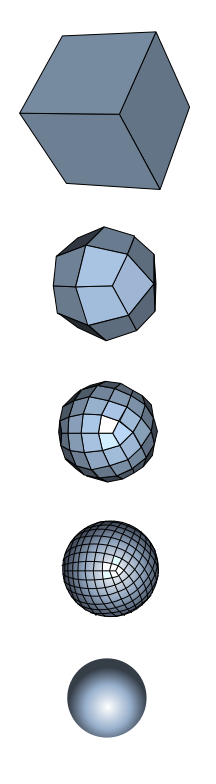
\includegraphics[width=15mm]{subdivisionSurface/catmull.png}

    \end{figure}
  \end{textblock*}
  
%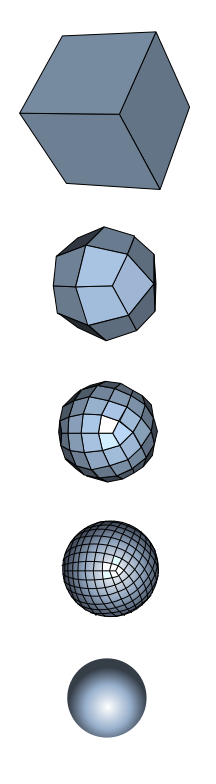
\includegraphics[height=130px]{subdivisionSurface/catmull.png}
 \end{minipage} \hfill %<-  si tu mets < à 1 au total
 \begin{minipage}[b]{0.88\linewidth}
\begin{block}{Algorithme récursif}
\small
\begin{itemize}

    \item<1->{Pour chaque surface :} ajouter un \textit{point de face}              \newline (moyenne des 4 \textit{points originaux}),
    \item<2->{Pour chaque arête :} ajouter un \textit{point d'arête}                \newline (moyenne des 2 \textit{points de face} et des 2 \textit{points originaux}),
    \item <3->Relier les \textit{points de face} créés aux \textit{points d'arête} correspondant,
    \item<4->{Pour chaque \textit{point original} P :} 
        \begin{itemize}
        \item<5-> considérer toutes les faces qui touchent P 
            \newline et calculer la position moyenne \textbf{F} de leur \textit{point de face},
        \item <6->considérer toutes les arêtes qui touchent P 
            \newline et calculer la position moyenne \textbf{A} des milieux de chaque arête,
        \item<7-> déplacer P au barycentre de ces positions 
        $\frac{F +2A + (n-3)P}{3}$
        \end{itemize}
    
    \item <8->Modifier les points originaux $\rightarrow$ modifier leurs points d'arêtes.
   % \newline Relier les points obtenus aux nouveaux points d'arêtes.
    
    %\item définir les nouvelles faces déterminée par les arêtes
    \end{itemize}
\end{block}

\end{minipage} 

\end{frame}
%-----------------------------------------------------------------
\begin{frame}[c]{Modélisation par subdivisions de face}{Quel niveau choisir ?}
Pour un \textbf{quadrangle} et pour une subdivision de \textbf{niveau n} : 
\newline $\rightarrow$ \textbf{4n faces produites}
\newline
%Cette augmentation massive du nombre de faces (et de vertices) cause un ralentissement aussi bien à l’édition qu’au rendu, et souligne l’intérêt d’un plus faible niveau de Subsurf pour l’édition que pour le rendu.
%il y a aussi triangulaire  3 × 4n-1.mais mailleur rendu avec quadra
\begin{block}{Pourquoi ne pas choisir le niveau le plus élevé ?}
\begin{itemize}
\item{Résolution de l’écran}
\item{Temps de chargement + Mémoire système}
\item{Objet éloigné $\rightarrow$ bas niveau}
\end{itemize}
\end{block}
\end{frame}
%-----------------------------------------------------------------

%------------Modélisation par surfaces implicites---------------
\subsection{Modélisation par surfaces implicites}
\begin{frame}[c]{Modélisation par surfaces implicites}{Primitives implicites : Surface équipotentielle}
\begin{itemize}
\item<1->  $\ne$ modèles paramétriques (coordonnées des points)
\item<1-> Pas représentées explicitement : $f(x,y,z)=0$
\item<1-> \textit{Sphère : $f(x,y,z)=x^2 + y^2 +z^2 +1$}
\newline
\item<2-> Réduitent à  $\mathbb{R}^3$ pour la modélisation de formes
\item<2-> Le formalisme implicite définit une surface comme un ensemble de points de l’espace vérifiant une propriété
\item <2->Liée à la valeur prise en ces points par une fonction
\newline F : $\mathbb{R}^3 \rightarrow \mathbb{R}$ on associe un scalaire à tout point de l'espace
\end{itemize}
\end{frame}
%-----------------------------------------------------------------


%-----------------------------------------------------------------
\begin{frame}[c]{Modélisation par surfaces implicites}{Primitives implicites : Surface équipotentielle}
\begin{itemize}
\item Surface S définie comme l’\textit{iso-surface} de l'\textit{iso-valeur} fixée par la fonction F : $S=\{P \in\mathbb{R}^3 / F(P)=iso\}$
\begin{itemize}
\item la fonction implicite
\item le champ scalaire
\item la fonction de potentiel %(analogie avec les champs électromagnétiques étudiés en physique)
\end{itemize}
\end{itemize}
\begin{center}
\begin{figure}
%\onslide<5->
\parbox{5cm}{\caption{A chaque \textit{iso-valeur} correspond une \textit{iso-surface}}}
\parbox{6cm}{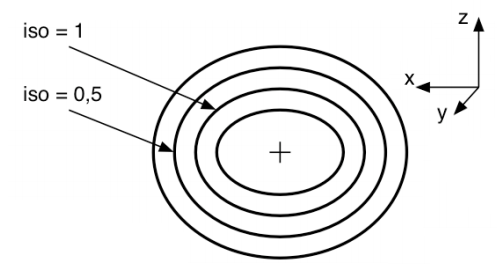
\includegraphics[width=4.3cm]{surfaceImplicite/iso.png}}
\end{figure}

\end{center}
\end{frame}



%-----------------------------------------------------------------
\begin{frame}[c]{Modélisation par surfaces implicites}{Primitives implicites : Surface équipotentielle}

\begin{itemize}
\item S fermée $\rightarrow$ sépare l'espace en 2 (extérieur / intérieur)
\item Connaître la position du point par rapport à la surface frontière
\item Avec un potentiel strictement décroissant, position de P :
    \begin{itemize}
    \item Si F(P) > iso, le point P est à l'intérieur de la surface,
    \newline \textbf{(Volume implicite / équipotentiel)}
    \item Si F(P) = iso, le point P est sur la surface,
    \item Si F(P) < iso, le point P est à l’extérieur de la surface
    \end{itemize}
\end{itemize}

\end{frame}

\begin{frame}[c]{Modélisation par surfaces implicites}{Volumes / Surfaces implicites}
\begin{block}{Primitive implicite à squelette ponctuel}
 \begin{itemize}
 \item d’un centre $Q_i $
 \item d’une fonction de densité $F_i$
 \end{itemize}
 	 
\end{block}
Scène composée de n primitives 
\newline $\Rightarrow$ forme complexe (volume ou surface implicite)
\begin{block}{Fonction de densité globale $F$}
\begin{itemize}
\item Mélange : $F(P) = \sum_{i=1}^{n} (F_i(P))$
\item Union : $\cup (F_1, F_2, ..., F_n)(P) = max(F_1(P), F_2(P), ..., F_n(P))$
\item Intersection : $\cap (F_1, F_2, ..., F_n)(P) = max(F_1(P), F_2(P), ..., F_n(P))$
\item Appliquer des fonctions
\end{itemize}
\end{block}

\begin{center}
\begin{figure}
%\onslide<5->
\parbox{2cm}{\caption{Mélange}}
\parbox{1.8cm}{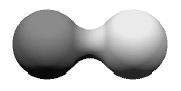
\includegraphics[width=1.8cm]{surfaceImplicite/melange.png}}
\hfill
\parbox{2cm}{\caption{Intersection}}
\parbox{1.3cm}{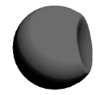
\includegraphics[width=1.3cm]{surfaceImplicite/intersection.png}}
\end{figure}

\end{center}
\end{frame}

\begin{frame}[c]{Modélisation par surfaces implicites}{Volumes / Surfaces implicites}
    \begin{itemize}
        \item Influence de l'iso-valeur
    \end{itemize}
\begin{center}
    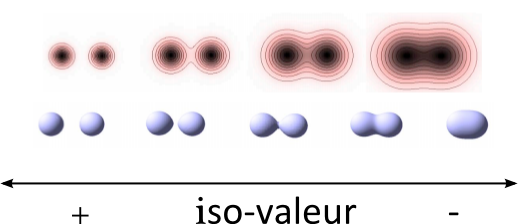
\includegraphics[width=4.3cm]{surfaceImplicite/influence.png}
\end{center}

    \begin{block}{Avantage}
        \begin{itemize}
            \item Contrôle sur la continuité et la dérivabilité des surfaces obtenues
\newline $\Rightarrow$ réaliser la jonction de deux objets sans une arête vive mais par une surface lisse.
        \end{itemize}

    \end{block}
\end{frame}

%----------------------------Modélisation par géometrie------------
\subsection{Modélisation par géométrie de construction de solides}
\begin{frame}[c]{Modélisation par géométrie de construction de solides}{Méthodes}

\begin{block}{2 méthodes}


\begin{itemize}
\item \textbf{CSG} ("Constructive Solid Geometry" dite aussi "modélisation solide" ou "modélisation volumique"),
\item \textbf{B-Rep} ("Boundary Representation" ou "modélisation surfacique").
\end{itemize}

\end{block}
\end{frame}
%----------------------------------------

\begin{frame}[c]{Modélisation par géométrie de construction de solides}{Modélisation volumique}

\begin{itemize}
\item Combinaison d'objets solides simples
\newline \textit{cylindre, sphère, cône,...}
\end{itemize}
\newline
\begin{itemize}
\item Transformations géométriques
\newline \textit{translation, rotation, homothétie}
\end{itemize}
\newline
\begin{itemize}
\item Utilisation d'opérateurs géométriques booléens
\newline \textit{union, soustraction, intersection,...}
\end{itemize}

  \begin{textblock*}{30mm}[0,0](90mm,20mm)
    \begin{figure}
    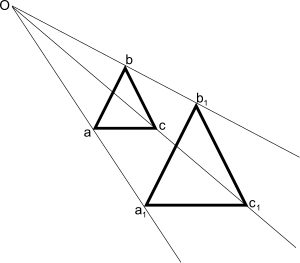
\includegraphics[width=25mm]{geo/homothetie.png}
    \caption{Homothétie}
    \end{figure}
  \end{textblock*}

\begin{center}


\begin{figure}
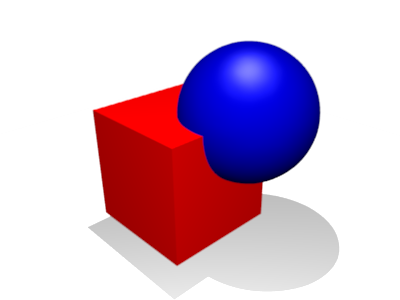
\includegraphics[width=25mm]{geo/geoUnion.PNG}
\hfill
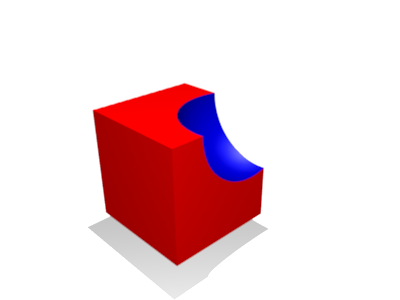
\includegraphics[width=25mm]{geo/geoDifference.PNG}
\hfill
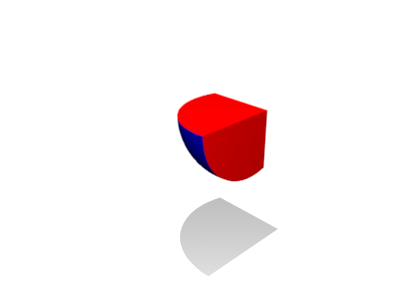
\includegraphics[width=25mm]{geo/geoIntersection.PNG}
\caption{Transformations}
\end{figure}


\end{center}
\end{frame}


%---------------------------------------------------------
\begin{frame}[c]{Modélisation par géometrie de construction de solides}{Modélisation volumique : Structure}
\begin{itemize}
\item <1->Stockée sous forme arborescente 
\newline (description des opérations et des éléments manipulés)
\item <1->Facilite les modifications
\end{itemize}
\newline
\begin{center}
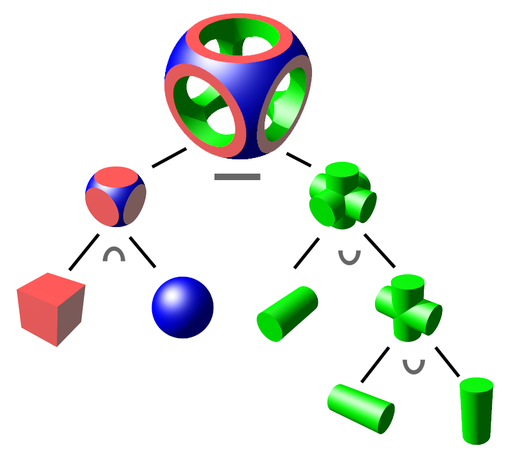
\includegraphics[width=65mm]{geo/geoStructure.png}
\end{center}
\newline


\end{frame}

%-----------------------------------------------------------------
%---------------------------------------------------------
\begin{frame}[c]{Modélisation par géometrie de construction de solides}{Modélisation volumique : Structure}

\newline

\begin{block}<1->{Avantages}
    \begin{itemize}
    \item Frontières parfaites et non approchées pour les volumes complexes         \newline ($\ne$ techniques à base de polygones)
    \newline
    \item Optimisation/accélération des calculs : 
    \newline basés sur des volumes plutôt que sur les polygones
    \newline \textit{(calculs de projection, calculs de collision entre deux solides)}
    %oral :  plus rapide de projeter un polygone formé par les arêtes d'un solide que de projeter les polygones du solide}
     %oral : collision... convexes sont très rapides, il suffit de tester si au moins un des deux a un point inclus dans l'autre.}
    \end{itemize}
\end{block}
\newline
\begin{block}<2->{Inconvénients}
     \begin{itemize}
    \item Liberté de modélisation restreinte 
    % oral : par les possibilités de créer le volume désiré par un ensemble d'opérations. De plus les formes présentes dans le monde réel sont peu ou pas géométriques et même un ballon n'est pas parfaitement sphérique lorsqu'il est posé sur le sol.
    \newline
    \item Hiérarchies d'opérations très complexes 
    %oral : qui vont alourdir les calculs de rendu.
%Le nombre de primitives disponibles va directement influer sur l'algorithme de rendu car ce dernier doit savoir les prendre toutes en compte ce qui peut alourdir son écriture.
     \end{itemize}
\end{block}

\end{frame}

%-----------------------------------------------------------------

\begin{frame}[c]{Modélisation par géometrie de construction de solides}{Modélisation surfacique}
\begin{itemize}
\item Représenter la peau des objets géométriques en "cousant" des carreaux géométriques restreints, portés par des surfaces canoniques %(en général des surfaces B-splines, des Bézier, des NURBS)
\newline
\item Représentation dans laquelle un solide est entièrement représenté par son bord (constitué de faces, arêtes et sommets) 
\end{itemize}




\end{frame}
%-----------------------------------------------------------------


\section{Blender}

\subsection{Présentation de Blender}

\begin{frame}[c]{Présentation de Blender}{Introduction}
\begin{block}{Imagerie de synthèse}
\begin{itemize}
\item Modélisation d'un objet
\item Mise en couleurs (matériaux et textures)
\item Eclairage
\item Rendu
\item Animation
\end{itemize}
\end{block}
\newline
\begin{center}
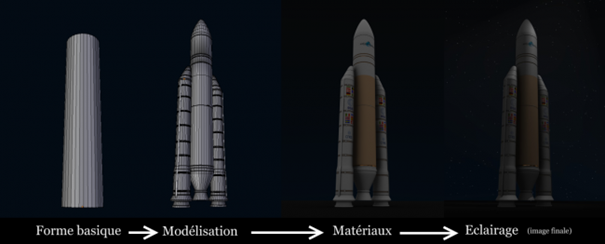
\includegraphics[width=65mm]{presentationBlender/process.png}
\end{center}
\end{frame}

\begin{frame}[c]{Présentation de Blender}{Caractéristiques}
    \begin{block}{Caractériqtiques}
        \begin{itemize}
            \item Modeleur intuitif et performant
            \item Méthodes d'animation multiples %(Ikey, armature…)
            \item Blender Game
            %\item Flou de mouvement et flou focal 
            \item Formats d'import/export variés %afin d'utiliser votre travail dans d'autres logiciels ;
%\item Système de nodes, afin d'améliorer son image sans passer par un logiciel 2D 
            \item Simulation de fluides %, pour créer des jets d'eau en tout sens ;
            \item Softbodies, moteur physique 
            \newline(simuler les collisions et déformations d'objets)
            \item Interface personnalisable 
            \item Rendus externes possibles (YafaRay, Indigo…) \newline(générer une image plus réaliste)
            
            %YafaRay utilise la méthode de l'illumination globale pour produire des rendus réalistes de scènes 3D.
            \item Scripteur Python (permet de créer de petits plugin)
        \end{itemize}
    \end{block}
\end{frame}

\begin{frame}[c]{Présentation de Blender}{Avantages / Inconvénients}
%comparaison gimp 2D

    \begin{block}{Avantages}
        \begin{itemize}
            \item Logiciel \textbf{libre} et \textbf{gratuit} %open source
            \item Léger : environ 20 Mo
            \item Portabilité : Windows, Linux, Mac OS X
            \item Performant
            %en plus des outils de base :
            \item Visualisateur d'images, éditeur vidéo, module dédié à la création et l'exécution de jeux (Blender Game)
        \end{itemize}
    \end{block}

    \begin{block}{Inconvénients}
        \begin{itemize}
            \item Difficile d'utilisation au début
        \end{itemize}
    \end{block}
\end{frame}

\subsection{L'interpréteur python}

\begin{frame}{Blender}{Interpréteur Python}
    \begin{block}{Généralités}
    \begin{itemize}
    \item{
        Blender possède un interpréteur python.    
    }
    \item{
        Pour gérer toute la partie animation/rendu 3d...
    }
    \item{
        Pour modéliser par l'intermédiaire d'algorithme, les formes 3d désirées.
    }
    \item{
        Une grande documentation est présente sur le site de blender.org
    }
    \item{
        Launcher pour les scripts depuis le menu principal de blender, pour une interaction intuitive
    }
    \end{itemize}
    \end{block}
\end{frame}

\begin{frame}{Blender}{Interpréteur Python}
    \begin{itemize}
        \item{
        Vous pouvez accéder à l'interpréteur depuis le menu outils.\\
        }
        \newline
        \begin{center}
        \includegraphics<1>[height=180px]{Python/MenuPython.png}
        \end{center}
    \end{itemize}
\end{frame}

\begin{frame}{Blender}{Interpréteur Python}
    \begin{itemize}
        \item{
        Lorsque vous lancez l'interpréteur, une petite fenêtre va s'ouvrir en haut à droite, que vous pourrez  agrandir à loisirs.\\
    }
    \newline
        \includegraphics<1>[width=300px]{Python/fenetre.png}
    \end{itemize}
\end{frame}

\begin{frame}{Blender}{Interpréteur Python}
    \begin{itemize}
        \item{Il existe depuis Blender, un accès à la documentation relative à python et aux scripts, depuis le menu Aide.\\
        }
        \newline
        \includegraphics<1>[width=300px]{Python/MenuPythonDoc.png}
    \end{itemize}
\end{frame}

\begin{frame}{Blender}{Interpréteur Python}
    \begin{itemize}
        \item{
        La documentation du python est présente sur le site de Blender.\\
        }
        \newline
        \includegraphics<1>[width=300px]{Python/BlenderDocumentation.png}
    \end{itemize}
\end{frame}


\subsection{Rendu 3D}


\begin{frame}{Blender}{Rendu 3D}
    \begin{block}{Points Clés}
    \begin{itemize}
        \item{
        Le rendu 3D est l'étape finale d'un projet sur Blender, c'est le moment où tocontrollerjet va être testé.
        }
        \item{
        En fonction de la taille du projet, il est possible que vous ayez quelques soucis de puissances.
        }
        \item{
        Il existe un système, permettant de diviser le travaille demandé au(x) processeur(s), entre plusieurs machines, le $ render farm $.
        }
    \end{itemize}
    \end{block}
\end{frame}

\begin{frame}{Blender}{Rendu 3D}
    \begin{block}{Comment contrôler le rendu}
    \begin{itemize}
        \item     Output        \\
        \item     Render Layer  \\
        \item     Render        \\
        \item     Anim          \\
        \item     Baking        \\
        \item     Format        \\
        \item     Stamp         \\
    \end{itemize}
    \end{block}
\end{frame}

\begin{frame}{Blender}{Rendu3D}
    \begin{block}{Les étapes pour un rendu optimisé}
    \begin{itemize}
        \item   Créer les images \\
        \item   Éclairer la scène \\
        \item   Premier rendu, qui optimise le temps de calcul \\
        \item   Régler et ajuster l'éclairage et les matériaux \\
        \item   Répéter les étapes précédentes \\
        \item   Sauvegarde  \\
         
    \end{itemize}
    \end{block}
\end{frame}

\begin{frame}{Blender}{Rendu3D}
  
    \begin{block}{3 outils de rendu}
      \begin{itemize}
        \item   Le moteur de rendu\\
        \item   Compositing\\
        \item   Montage\\
    \end{itemize}
    \end{block}
    
 
   
  
\end{frame}

\begin{frame}{Blender}{Rendu3D}
    \begin{block}{Optimisation du temps de calcul}
    \begin{itemize}
        \item{
            Blender consomme beaucoup de ressources en particulier sur le CPU, mais des solutions vous sont proposées afin d'optimiser les calculs.
        }    
        \\
        \item{
            Si vous possédez un multicoeur, vous pouvez augmenter le nombre de thread afin d'utiliser tous vos coeurs dans les calculs.
        }
        \\
        \item{
            Si vous possédez plusieurs ordinateurs, sur un même LAN, vous pouvez partager le travail entre les différentes machines.\\
          \begin{itemize}
          \item Passer le dossier contenant tous les fichiers de votre projet,
          \item Lancer le logiciel Blender sur chaque machine,
          \item Ouvrir ce projet.
          \end{itemize}  
            
            Si vous passez par le chemin relatif, toutes les modifications seront automatiquement enregistrées sur le fichier original.
        }
    \end{itemize}
    \end{block}
\end{frame}



\subsection{Sources}

\begin{frame}{Sources}
    \begin{block}{Sources}
    \begin{itemize}

        \item{   www.blender.org }
        \item{   www.wiki.blender.org }

    \end{itemize}
        \end{block}

    
\end{frame}


% Placing a * after \section means it will not show in the
% outline or table of contents.
%\section*{Summary}


\end{document}


 